\documentclass[letterpaper,12pt]{article}
\usepackage{epsfig,latexsym,amsmath,amssymb,epic,eepic,psfrag,subfigure,float,euscript,array}
\usepackage[latin1]{inputenc}
\usepackage{standalone}
\usepackage{tikz,pgf,pgfplots}
\usepackage[margin=2.5cm]{geometry}

\newenvironment{exercise}[1][Uppgift]{\begin{trivlist} \item[\hskip
    \labelsep {\stepcounter{exerctr}\bfseries #1
      \arabic{exerctr}}]}{\end{trivlist}\vspace{10mm}}

\newcounter{exerctr}
\newcounter{abcctr}[exerctr]

\newcommand{\abc}{\noindent\vspace{1mm}\\ {\bf
    \stepcounter{abcctr}(\alph{abcctr})\ }}
\newcommand{\bbm}{\begin{bmatrix}}
\newcommand{\ebm}{\end{bmatrix}}
\newcommand{\point}[1]{\hfill {\bf (#1p)}\\ \vspace{-5mm}}
\newcommand{\ctrb}{\EuScript{S}}
\newcommand{\Lap}{\mathcal{L}}
\newcommand{\obsv}{\EuScript{O}}
\newcommand{\realdel}[1]{\text{Re}\left\{#1\right\}}
\newcommand{\imagdel}{\text{Im}}
\newcommand{\bC}{\mathbb{C}}
\newcommand{\bR}{\mathbb{R}}
\newcommand{\bmpv}{\begin{minipage}[t]}
\newcommand{\bmps}{\begin{minipage}[t]{45mm}}
\newcommand{\bmpm}{\begin{minipage}[t]{90mm}}
\newcommand{\bmpl}{\begin{minipage}[t]{\textwidth}}
\newcommand{\emp}{\end{minipage}}
\newcommand*{\zethree}{\big(z - \mexp{-3h}\big)}
\newcommand*{\mexp}[1]{\ensuremath{\mathrm{e}^{#1}}}

\newcommand*\circled[1]{\tikz[baseline=(char.base)]{
            \node[shape=circle,draw,inner sep=2pt] (char) {#1};}}


\DeclareMathOperator{\shift}{q}

\addtolength{\topmargin}{-1cm}
\textheight 23.5cm
%\oddsidemargin 0.61cm
%\evensidemargin 0.61cm


\title{Computerized Control Final Exam (31\%)}
\author{Kjartan Halvorsen}
\date{May 5 2017}
\begin{document}

\maketitle


\begin{description}
\item[Time] 2017-05-05 16:00 - 19:00
\item[Place] 5105
\item[Permitted aids] The single colored page with your own notes, table of transforms, calculator
\end{description}

All answers should be \textbf{readable and well motivated} (if nothing else is written). Solutions/motivations should be written on the provided spaces in this exam. Use the last page if more space is needed.

\begin{center}
{\Large Good luck!} \\
\end{center}

\noindent
\fbox{
\bmpl
{\bf Matricula and name:}\\
\vspace*{30mm}
\emp}

\clearpage

%-----------------------------------------------------------------


\subsection*{Problem 1 (70p)}
Figure \ref{fig:magnetic-suspension} shows a simple, one-dimensional magnetic suspension system. The current $i$ in the windings generates a magnetic field which suspends the mass $m$. Ignoring friction, there are two forces acting on the mass: gravity and the magnetic force. The magnetic force is proportional to the square of the current $i$ and inverse proportional to the square of the gap distance $x$. This gives the equation of motion 
\begin{equation}
m \ddot{x} = -C \left( \frac{i}{x} \right)^2 + mg.
\end{equation}
\begin{figure}[htb]
\begin{center}
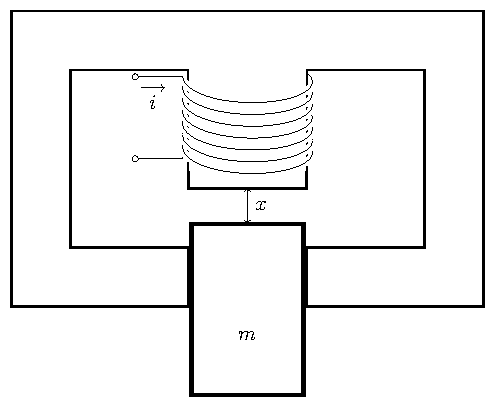
\includegraphics[width=0.5\linewidth]{./magnetic-suspension}
\caption{A magnetic suspension system. The force of gravity acts to pull the mass $m$ downwards. The force due to the magnetic field generated by the current $i$ keeps the mass from falling down. }
\label{fig:magnetic-suspension} 
\end{center}
\end{figure}
The system is non-linear, so in order to use linear control design, the system must be linearized about an operating point. Introduce the variations \(y\) and \(u\) about the operating point
\begin{align*}
x &= x_0 + y \\
i &= i_0 - \tilde{i}.
\end{align*}
The input signal to the system \eqref{eq:ode} is the change  \(\tilde{i}\) in the current in the windings, and the output signal is the change \(y\)  in the gap distance. The negative sign in the variation \(i = i_0 - \tilde{i}\) is introduces so that a positive input signal leads to a positive change in the gap distance. With operating point \[\frac{i_0}{x_0} = \sqrt{\frac{mg}{C}},\] the linearized model becomes
\begin{equation}
\ddot{y} = \frac{2g}{x_0} y + \frac{2 \sqrt{Cg}}{\sqrt{m} x_0} u
\label{eq:ode}
\end{equation}
with transfer function
\begin{equation}
G(s) = \frac{ \frac{ 2\sqrt{Cg} }{\sqrt{m} x_0} }{s^2 - \frac{2g}{x_0}}.
\end{equation}
The system is unstable, with poles in \(\pm \sqrt{\frac{2g}{x_0}}\). Normalizing the time (using the unit of time \(T=\sqrt{\frac{x_0}{2g}}\)) and setting $u(t) = \frac{2\sqrt{Cg}}{\sqrt{m}x_0} \tilde{i}(t)$ gives the plant model
\begin{equation}
Y(s) = G(s)U(s) = \frac{1}{s^2 - 1} U(s).
\label{eq:trf}
\end{equation}

\subsubsection*{(a)}
% Discretize
Show that discretizing the model \eqref{eq:trf} using zero-order-hold with $h=0.1$ gives the discrete-time pulse transfer function
\begin{equation}
H(z) = 5.0\cdot 10^{-3} \frac{z+1}{z^2 - 2.01z +1}.
\end{equation}
and plot the zeros and poles of the system in the z-plane.
 
\noindent
\fbox{
   \bmpl
   {\bf Solution:}\\
   \vspace*{135mm}
   \emp}
 
\subsubsection*{(b)}
The magnetic suspension system is to be stabilized using the control law
\begin{equation}
 U(z) = K \frac{z - 0.9}{z} E(z) = K \frac{z - 0.9}{z}  \big(Y(z) - Y_{ref}(z)\big). 
\label{eq:controllaw}
\end{equation}
Write the control law as a difference equation. Explain also which values must be stored in the computer between sampling instants in order to calculate the control signal.
 
\noindent
\fbox{
   \bmpl
   {\bf Solution:}\\[3mm]

   \vspace*{115mm}

   \( u(k+1) = \)\\[3mm]
   \emp}
 

\newpage
\subsubsection*{(c)}

With the control law \eqref{eq:controllaw}, we obtain the below root locus for the closed-loop poles. Explain briefly (3-5 sentences) the closed-loop behaviour of the system for different values of the feedback gain $K$.
\begin{center}
\begin{tikzpicture}
\node {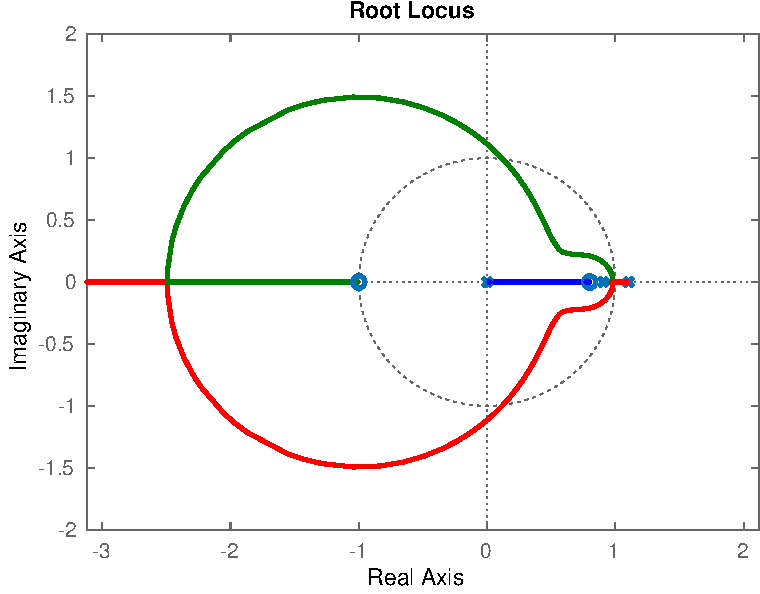
\includegraphics[width=0.7\linewidth]{final_p1_rlocus_vt17-crop}};
\node[ pin=60:{$K=190$}] at (1.78,2.0) {};
\node[ pin=60:{$K=5$}] at (3.4,0.1) {};
\end{tikzpicture}
\end{center}

\noindent
\fbox{
   \bmpl
   {\bf Answer:}\\
   \vspace*{75mm}
   \emp}
 

\newpage
\subsubsection*{(d)}

Figure~\ref{fig:step} shows four different step-responses, obtained with different values for the gain parameter $K$. Match the step-response to the gain. Motivate!

\noindent
\fbox{
\bmpl
{\bf Answer and motivation:}\\[3mm]
{\large
\begin{tabular}{|l|c|c|c|c|}
\hline
Gain & $K=6$ & $K=54$ & $K=180$ & $K=200$\\ \hline
Response & & & &\\\hline
\end{tabular}
}\vspace*{100mm}
\emp}



\begin{figure}[tp]
\begin{center}
\begin{tabular}{cc}
A & B\\
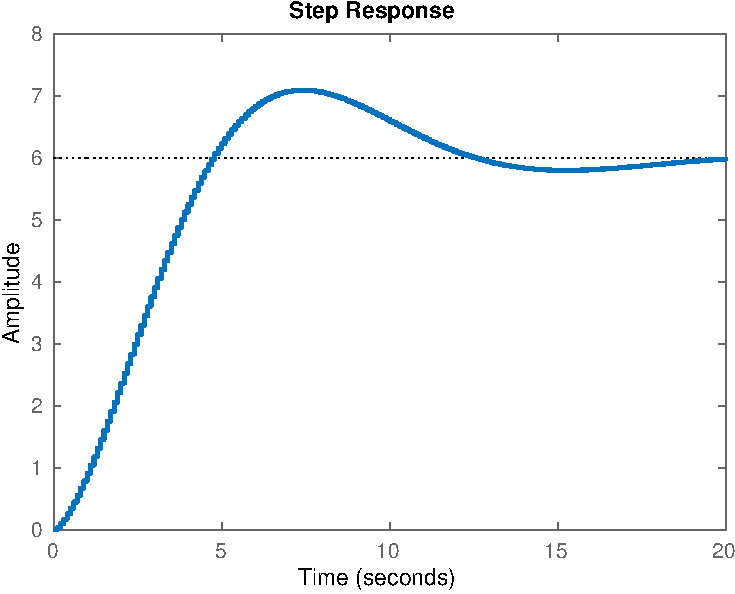
\includegraphics[width=0.4\linewidth]{step-plot-1-vt17-crop}
&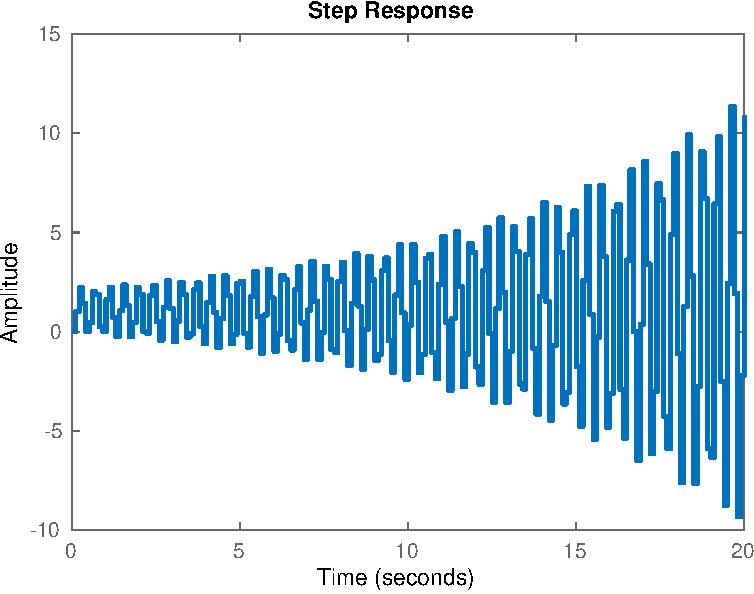
\includegraphics[width=0.4\linewidth]{step-plot-4-vt17-crop}\\
C & D\\
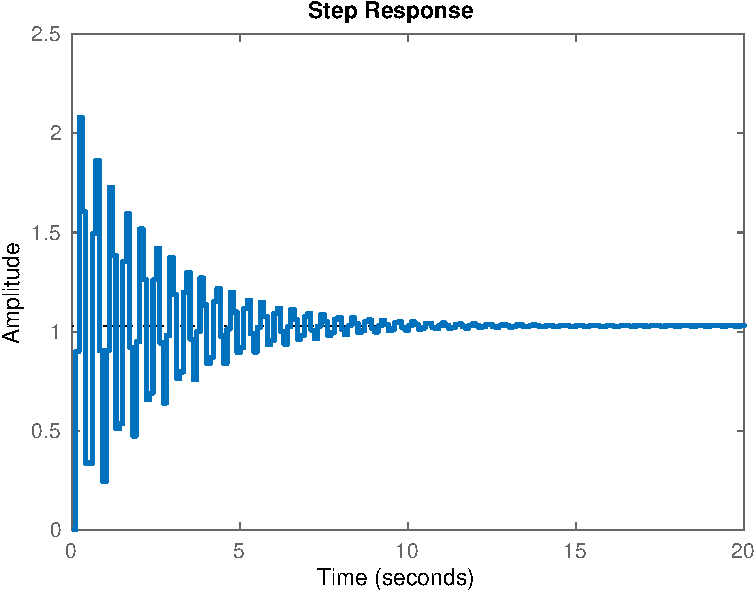
\includegraphics[width=0.4\linewidth]{step-plot-3-vt17-crop}
&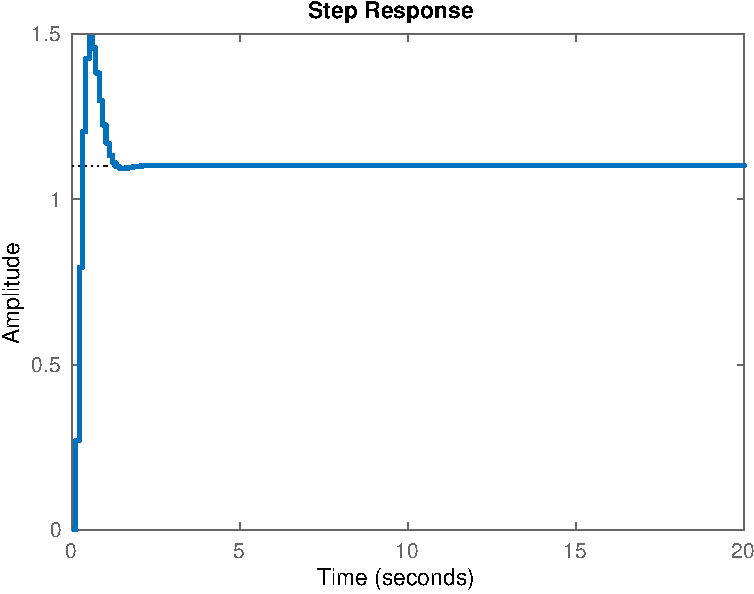
\includegraphics[width=0.4\linewidth]{step-plot-2-vt17-crop}

\end{tabular}
\caption{Step responses, problem 1 (d).}
\label{fig:step}
\end{center}
\end{figure}


\cleardoublepage

\subsection*{Problem 2 (30p)}

The normalized magnetic suspension system can be represented on state-space form as
\begin{equation}
\begin{split}
x(k+1) &= \bbm 2.01 & -1\\1 & 0 \ebm x(k) + \bbm 1\\0\ebm u(k)\\
y(k) &= 5\cdot 10^{-3} \bbm 1 & 1 \ebm x(k)
\end{split}
\end{equation}

\subsubsection*{(a)}

Show that the system is reachable.

\noindent
\fbox{
\bmpl
{\bf Solution:}\\
\vspace*{120mm}
\emp}



\subsubsection*{(b)}

Determine the state feedback gain 
\[ u(k) = u_c(k) - l_1 x_1(k) - l_2 x_2(k) \]
which gives a closed-loop system with poles in the origin. What is a controller with this choice of closed-loop poles called?

\noindent
\fbox{
\bmpl
{\bf Controller design:}\\
\vspace*{160mm}
\emp}



\cleardoublepage

\noindent
{\bf If necessary,} you can continue your solutions on this sheet. Mark clearly which problem the solution corresponds to.

%\end{document}

\section*{Solutions}
\subsection*{Problem 1}

\subsubsection*{(a)}
The step-response of the system is 
\begin{equation*}
\begin{split}
Y(s) &= \frac{1}{(s+1)(s-1)s} = \frac{\frac{1}{2}}{s+1} + \frac{\frac{1}{2}}{s-1} - \frac{1}{s}\\
y(t) &= \frac{1}{2} \mathrm{e}^{-t} + \frac{1}{2} \mathrm{e}^{t} - u_H(t)\\
y(kh) &= \frac{1}{2} \left(\mathrm{e}^{-h}\right)^k + \frac{1}{2} \left(\mathrm{e}^{h}\right)^k - u_H(k)\\
\end{split}
\end{equation*}
Taking the z-transform gives
\begin{equation*}
\begin{split}
Y(z) &= \frac{\frac{1}{2}z}{z - \mathrm{e}^{-h}} + \frac{\frac{1}{2}z}{z - \mathrm{e}^{h}} - \frac{z}{z-1}.
\end{split} 
\end{equation*}
Dividing with the z-transform of the unit step \(\frac{z}{z-1}\) gives
\begin{equation*}
\begin{split}
H(z) &= \frac{Y(z)}{U(z)} = \frac{\frac{1}{2}(z-1)}{z - \mathrm{e}^{-h}} + \frac{\frac{1}{2}(z-1)}{z - \mathrm{e}^{h}} - 1 \\
&= \frac{ \frac{1}{2} (z-1)(z-\mathrm{e}^{h}) + \frac{1}{2}(z-1)(z - \mathrm{e}^{-h}) - (z-\mathrm{e}^{-h})(z - \mathrm{e}^h)}{(z-\mathrm{e}^{-h})(z - \mathrm{e}^h)}\\
&= \frac{ \frac{1}{2}z^2 - \frac{1}{2}(1+\mathrm{e}^{h})z + \frac{1}{2}\mathrm{e}^{h} + \frac{1}{2}z^2 -\frac{1}{2}(1 + \mathrm{e}^{-h})z + \frac{1}{2}\mathrm{e}^{-h} - z^2 + (\mathrm{e}^{-h} + \mathrm{e}^{h})z - 1}{(z-\mathrm{e}^{-h})(z - \mathrm{e}^h)}\\
&= \frac{ (-\frac{1}{2} -\frac{1}{2}\mathrm{e}^h - \frac{1}{2} - \frac{1}{2}\mathrm{e}^{-h} + \mathrm{e}^{-h} + \mathrm{e}^h) z + (\frac{1}{2}\mathrm{e}^h + \frac{1}{2}\mathrm{e}^{-h} - 1)}{z^2 - (\mathrm{e}^{-h} + \mathrm{e}^{h})z + 1}\\
&= \frac{ (\frac{1}{2}(\mathrm{e}^{h} + \mathrm{e}^{-h}) - 1) (z+1)}{z^2 - (\mathrm{e}^{-h} + \mathrm{e}^{h})z + 1}.
\end{split}
\end{equation*}
Inserting \(h = 0.1\) gives
\[ H(z) = 5.0\cdot 10^{-3} \frac{z+1}{z^2 - 2.01z +1}.\]
\begin{center}
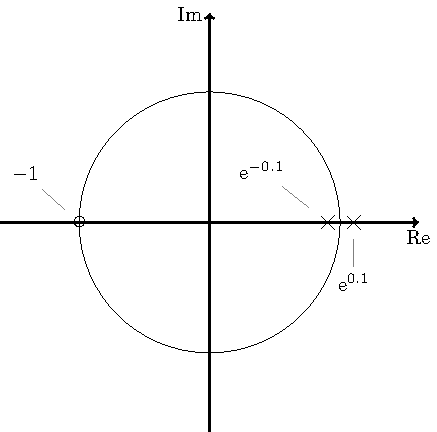
\includegraphics[]{imaginary-plane-pzmap}
\end{center}

\subsubsection*{(b)}
Using the shift operator we have
\begin{equation}
\begin{split}
  u(kh) &= K \frac{\shift - 0.9}{\shift} (y(kh) - y_{ref}(kh))\\
  \shift u(kh) &= K (\shift - 0.9) (y(kh) - y_{ref}(kh)) \\
  u(kh+h) &= K \left( y(kh+h) - 0.9y(kh) - y_{ref}(kh+h) - 0.9y_{ref}(kh)\right).
   \end{split}
 \end{equation}
In order to calculate the control signal at time $kh+h$ we need to store the previous output signal $y(kh)$ and the previous set-point $y_{ref}(kh)$. 
 
\subsubsection*{(c)}
For small gains $K<5$ the system is unstable since one pole is outside the unit circle. When the gain increases from $K=5$, the system is stable and at first dominated by the two poles close to the unit circle. When $K$ increases further, these two poles break out into the imaginary plane, and the closed-loop system will have oscillations. The damping is quite good though, and the system response will be quite fast as the $K$ increases. When $K>190$ the poles break out of the unit circle and the system becomes unstable. 

\subsubsection*{(d)}
Base on the discussion in (c), we must have

\begin{center}
\begin{tabular}{|l|p{0.2\linewidth}|p{0.2\linewidth}|p{0.2\linewidth}|p{0.2\linewidth}|}
\hline
Gain & $K=6$ & $K=54$ & $K=180$ & $K=200$\\ \hline
Response & Slow, stable response, no oscillations: \textbf{A} & Fast, well damped response, since poles are far from unit circle:. \textbf{D} & Fast and oscillatory response, since poles are close to the unit circle: \textbf{C} & Unstable response: \textbf{B}\\\hline
\end{tabular}
\end{center}
\subsection*{Problem 2}

\subsubsection*{(a)}
Reachability is tested by forming the matrix
\begin{equation*}
\begin{split}
  W_r &= \bbm \Gamma & \Phi \Gamma \ebm = \bbm 1 &  2.01 \\0 & 1 \ebm 
\end{split}
\end{equation*}
and calculating the determinant
\[ \det W_r = 1 \neq 0 \]
so the system is reachable.

 
\subsubsection*{(b)}

With the feedback \[u(k) = u_c(k) - l_1 x_1(k) - l_2 x_2(k) = u_c(k) - Kx(k) \]
inserted into the state-space model we get the closed-loop state space model
\begin{equation*}
\begin{split}
x(k+1) = \left(\Phi - \Gamma L\right)x(k) + \Gamma u_c(k)
\end{split}
\end{equation*}
which have poles given by the characteristic equation of $\Phi - \Gamma L$
\[ \det \left(zI - (\Phi - \Gamma L)\right) = 0. \] We have
\[ \Gamma L = \bbm l_1 & l_2\\ 0 & 0 \ebm \] and
\[ \Phi - \Gamma L = \bbm -2.01 -l_1 & 1-l_2\\1 & 0 \ebm \] which gives
\begin{equation*}
\begin{split}
\det \left(zI - (\Phi - \Gamma L)\right)  &= \det \bbm z +2.01 + l_1 & -1 + l_2\\-1 & z \ebm\\
  &= (z +2.01 + l_1)z + (-1+l_2)\\
&= z^2 + (2.01+l_1)z + (-1+l_2).
\end{split}
\end{equation*}
We want this characteristic polynomial to equal \(z^2\) which gives two poles in the origin. This gives the solution
\begin{align*}
l_1 &= -2.01\\
l_2 &= 1.\\
\end{align*}

\end{document}
